% ******************************* PhD Thesis Template **************************
% Please have a look at the README.md file for info on how to use the template

\documentclass[a4paper,12pt,customfont,numbered,print,index]{Classes/PhDThesisPSnPDF}

% ******************************************************************************
% ******************************* Class Options ********************************
% *********************** See README for more details **************************
% ******************************************************************************

% `a4paper'(The University of Cambridge PhD thesis guidelines recommends a page
% size a4 - default option) or `a5paper': A5 Paper size is also allowed as per
% the Cambridge University Engineering Deparment guidelines for PhD thesis
%
% `11pt' or `12pt'(default): Font Size 10pt is NOT recommended by the University
% guidelines
%
% `oneside' or `twoside'(default): Printing double side (twoside) or single
% side.
%
% `print': Use `print' for print version with appropriate margins and page
% layout. Leaving the options field blank will activate Online version.
%
% `index': For index at the end of the thesis
%
% `draftclassic': For draft mode without loading any images (same as draft in book)
%
% `draft': Special draft mode with line numbers, images, and water mark with
% timestamp and custom text. Position of the text can also be modified.
%
% `abstract': To generate only the title page and abstract page with
% dissertation title and name, to submit to the Student Registry
%
% `chapter`: This option enables only the specified chapter and it's references
%  Useful for review and corrections.
%
% ************************* Custom Page Margins ********************************
%
% `custommargin`: Use `custommargin' in options to activate custom page margins,
% which can be defined in the preamble.tex. Custom margin will override
% print/online margin setup.
%
% *********************** Choosing the Fonts in Class Options ******************
%
% `times' : Times font with math support. (The Cambridge University guidelines
% recommend using times)
%
% `fourier': Utopia Font with Fourier Math font (Font has to be installed)
%            It's a free font.
%
% `customfont': Use `customfont' option in the document class and load the
% package in the preamble.tex
%
% default or leave empty: `Latin Modern' font will be loaded.
%
% ********************** Choosing the Bibliography style ***********************
%
% `authoryear': For author-year citation eg., Krishna (2013)
%
% `numbered': (Default Option) For numbered and sorted citation e.g., [1,5,2]
%
% `custombib': Define your own bibliography style in the `preamble.tex' file.
%              `\RequirePackage[square, sort, numbers, authoryear]{natbib}'.
%              This can be also used to load biblatex instead of natbib
%              (See Preamble)
%
% **************************** Choosing the Page Style *************************
%
% `default (leave empty)': For Page Numbers in Header (Left Even, Right Odd) and
% Chapter Name in Header (Right Even) and Section Name (Left Odd). Blank Footer.
%
% `PageStyleI': Chapter Name next & Page Number on Even Side (Left Even).
% Section Name & Page Number in Header on Odd Side (Right Odd). Footer is empty.
%
% `PageStyleII': Chapter Name on Even Side (Left Even) in Header. Section Number
% and Section Name in Header on Odd Side (Right Odd). Page numbering in footer


% ********************************** Preamble **********************************
% Preamble: Contains packages and user-defined commands and settings
% ******************************************************************************
% ****************************** Custom Margin *********************************

% Add `custommargin' in the document class options to use this section
% Set {innerside margin / outerside margin / topmargin / bottom margin}  and
% other page dimensions
\ifsetCustomMargin
  \RequirePackage[left=37mm,right=30mm,top=35mm,bottom=30mm]{geometry}
  \setFancyHdr % To apply fancy header after geometry package is loaded
\fi

% Add spaces between paragraphs
%\setlength{\parskip}{0.5em}
% Ragged bottom avoids extra whitespaces between paragraphs
\raggedbottom
% To remove the excess top spacing for enumeration, list and description
%\usepackage{enumitem}
%\setlist[enumerate,itemize,description]{topsep=0em}

% *****************************************************************************
% ******************* Fonts (like different typewriter fonts etc.)*************

% Add `customfont' in the document class option to use this section

\ifsetCustomFont
  \usepackage{txfonts}
  % Set your custom font here and use `customfont' in options. Leave empty to
  % load computer modern font (default LaTeX font).
  %\RequirePackage{helvet}

  % For use with XeLaTeX
  %  \setmainfont[
  %    Path              = ./libertine/opentype/,
  %    Extension         = .otf,
  %    UprightFont = LinLibertine_R,
  %    BoldFont = LinLibertine_RZ, % Linux Libertine O Regular Semibold
  %    ItalicFont = LinLibertine_RI,
  %    BoldItalicFont = LinLibertine_RZI, % Linux Libertine O Regular Semibold Italic
  %  ]
  %  {libertine}
  %  % load font from system font
  %  \newfontfamily\libertinesystemfont{Linux Libertine O}
\fi

% *****************************************************************************
% **************************** Custom Packages ********************************

% ************************* Algorithms and Pseudocode **************************

%\usepackage{algpseudocode}


% ********************Captions and Hyperreferencing / URL **********************

% Captions: This makes captions of figures use a boldfaced small font.
%\RequirePackage[small,bf]{caption}

\RequirePackage[labelsep=colon,tableposition=top]{caption}
\renewcommand{\figurename}{Figure} %to support older versions of captions.sty


% *************************** Graphics and figures *****************************

%\usepackage{rotating}
%\usepackage{wrapfig}

% Uncomment the following two lines to force Latex to place the figure.
% Use [H] when including graphics. Note 'H' instead of 'h'
%\usepackage{float}
%\restylefloat{figure}

% Subcaption package is also available in the sty folder you can use that by
% uncommenting the following line
% This is for people stuck with older versions of texlive
%\usepackage{sty/caption/subcaption}
\usepackage{subcaption}

% ********************************** Tables ************************************
\usepackage{booktabs} % For professional looking tables
\usepackage{multirow}

%\usepackage{multicol}
%\usepackage{longtable}
%\usepackage{tabularx}


% *********************************** SI Units *********************************
\usepackage{siunitx} % use this package module for SI units


% ******************************* Line Spacing *********************************

% Choose linespacing as appropriate. Default is one-half line spacing as per the
% University guidelines

% \doublespacing
% \onehalfspacing
% \singlespacing


% ************************ Formatting / Footnote *******************************

% Don't break enumeration (etc.) across pages in an ugly manner (default 10000)
%\clubpenalty=500
%\widowpenalty=500

%\usepackage[perpage]{footmisc} %Range of footnote options


% *****************************************************************************
% *************************** Bibliography  and References ********************

%\usepackage{cleveref} %Referencing without need to explicitly state fig /table

% Add `custombib' in the document class option to use this section
\ifuseCustomBib
   \RequirePackage[square, sort, numbers, authoryear]{natbib} % CustomBib

% If you would like to use biblatex for your reference management, as opposed to the default `natbibpackage` pass the option `custombib` in the document class. Comment out the previous line to make sure you don't load the natbib package. Uncomment the following lines and specify the location of references.bib file

%\RequirePackage[style=numeric-comp, citestyle=numeric, sorting=none, natbib=true]{biblatex}
%\bibliography{References/references} %Location of references.bib only for biblatex

\fi

% changes the default name `Bibliography` -> `References'
\renewcommand{\bibname}{References}


% ******************************************************************************
% ************************* User Defined Commands ******************************
% ******************************************************************************

% *********** To change the name of Table of Contents / LOF and LOT ************

%\renewcommand{\contentsname}{My Table of Contents}
%\renewcommand{\listfigurename}{My List of Figures}
%\renewcommand{\listtablename}{My List of Tables}


% ********************** TOC depth and numbering depth *************************

\setcounter{secnumdepth}{2}
\setcounter{tocdepth}{2}


% ******************************* Nomenclature *********************************

% To change the name of the Nomenclature section, uncomment the following line

%\renewcommand{\nomname}{Symbols}


% ********************************* Appendix ***********************************

% The default value of both \appendixtocname and \appendixpagename is `Appendices'. These names can all be changed via:

%\renewcommand{\appendixtocname}{List of appendices}
%\renewcommand{\appendixname}{Appndx}

% *********************** Configure Draft Mode **********************************

% Uncomment to disable figures in `draft'
%\setkeys{Gin}{draft=true}  % set draft to false to enable figures in `draft'

% These options are active only during the draft mode
% Default text is "Draft"
%\SetDraftText{DRAFT}

% Default Watermark location is top. Location (top/bottom)
%\SetDraftWMPosition{bottom}

% Draft Version - default is v1.0
%\SetDraftVersion{v1.1}

% Draft Text grayscale value (should be between 0-black and 1-white)
% Default value is 0.75
%\SetDraftGrayScale{0.8}


% ******************************** Todo Notes **********************************
%% Uncomment the following lines to have todonotes.

%\ifsetDraft
%	\usepackage[colorinlistoftodos]{todonotes}
%	\newcommand{\mynote}[1]{\todo[author=kks32,size=\small,inline,color=green!40]{#1}}
%\else
%	\newcommand{\mynote}[1]{}
%	\newcommand{\listoftodos}{}
%\fi

% Example todo: \mynote{Hey! I have a note}

% ************Custom definitions
%\usepackage{txfonts}
%\usepackage{fontspec}
%\setmainfont[Path=/usr/share/fonts/truetype/calibri/,
%    BoldItalicFont=CalibriBI.ttf,
%    BoldFont      =CalibriB.ttf,
%    ItalicFont    =CalibriI.ttf]{Calibri.ttf}
\usepackage{xspace}
\usepackage{amsmath}
\usepackage{sty/ptdr-definitions}
\usepackage{longtable}
\usepackage{siunitx}

\newcommand\todo[1]{\textbf{#1}}
\newcommand{\metxy}{\ensuremath{E\!\!\!\!/_\text{x,y}}}
\newcommand{\sttbar}{\ensuremath{\sigma_{\ttbar}}\xspace}
\newcommand{\sttvis}{\ensuremath{\sigma_{\ttbar,\mathrm{vis}}\xspace}}
\newcommand{\mtt}{\ensuremath{m_{\ttbar}}\xspace}
\newcommand{\mtop}{\ensuremath{m_{\mathrm top}}\xspace}
\newcommand{\Wjets}{W+jets\xspace}
\newcommand{\Zjets}{Z+jets\xspace}
\newcommand{\ejets}{e+jets\xspace}
\newcommand{\mujets}{$\mu$+jets\xspace}
\newcommand{\ljets}{$\ell$+jets\xspace}
\newcommand{\mumu}{$\mu^+\mu^-$\xspace}
\newcommand{\ee}{$\mathrm{e^+e^-}$\xspace}
\newcommand{\mue}{$\mu^{\pm}\mathrm{e^{\mp}}$\xspace}
\newcommand{\pb}{\mbox{\ensuremath{\,\text{pb}}}\xspace}
\newcommand{\Pythia} {{\textsc{Pythia}}\xspace} %%%%%%%%%%%%%
\newcommand{\Powheg} {{\textsc{Powheg}}\xspace} %%%%%%%%%%%%%
\newcommand{\Herwig} {{\textsc{Herwig}}\xspace} %%%%%%%%%%%%%
\newcommand{\Herwigpp} {{\textsc{Herwig++}}\xspace} %%%%%%%%%%%%%
\newcommand{\MadSpin} {{\textsc{MadSpin}}\xspace} %%%%%%%%%%%%%
\newcommand{\MGaMCatNLO} {{\textsc{MG5\_aMC@NLO}}\xspace} %%%%%%%%%%%%%
\newcommand{\eepm}{\ensuremath{\Pep\Pem}}
\newcommand{\mmpm}{\ensuremath{\Pgmp \Pgmm}}
\newcommand{\ttpm}{\ensuremath{\Pgt^+ \Pgt^-}}
\newcommand{\empm}{\ensuremath{\Pepm \PGm^\mp}}
\newcommand{\pp}{\ensuremath{\Pp\Pp}}
\newcommand{\ppbar}{\ensuremath{\Pp\Pap}}
\newcommand{\ase}[2]{\ensuremath{_{~- #1}^{~+ #2}}}
\newcommand{\roots}{\ensuremath{\sqrt{s}}}
\newcommand{\lhcE}[1]{\ensuremath{\roots ={#1}~\TeV}}
%\newcommand{\PZ}{\ensuremath{\mathrm{Z}}}
\newcommand{\dy}{\ensuremath{\PZ/\Pgg^\star}}
\newcommand{\dyee}{\ensuremath{\dy\to\eepm}}
\newcommand{\dymm}{\ensuremath{\dy\to\mmpm}}
\newcommand{\dytt}{\ensuremath{\dy\to\ttpm}}
\newcommand{\mll}{\ensuremath{M_{\ell\ell}}\xspace}
\def\mrm{\mathrm}
\newcommand{\isocomb}{\ensuremath{I_\mrm{comb}}}
\newcommand{\WoZ}{\ensuremath{\PW/\PZ}}
\providecommand{\POWHEG} {\textsc{Powheg}\xspace}
\providecommand{\PYTHIA} {\textsc{Pythia}\xspace}
\providecommand{\HERWIGPP} {\textsc{Herwig++}\xspace}
\newcommand{\tW}{\ensuremath{\mathrm{t}\PW}}
\newcommand{\VV}{\ensuremath{\mathrm{VV}}}
\newcommand{\ns}{\ensuremath{\mrm{ns}}}
\newcommand{\wmn}{\ensuremath{\PW\to\Pgm\Pgngm}}
\newcommand{\met} {\ensuremath{E\!\!\!\!/_T}}
\renewcommand{\MET}{\mbox{$\not \!\! E_T$}}
\newcommand{\pythia}{{\sc{Pythia}}}
\renewcommand{\ttbar}{\ensuremath{\mathrm{t}\bar{\mathrm{t}}}\xspace}
\newcommand{\invpb}{pb$^{-1}$}
\newcommand{\geVcc}{GeV}
\providecommand{\ee}{\ensuremath{ee}\xspace}
\newcommand{\emu}{\ensuremath{\mathrm{e}^\pm\mu^\mp}\xspace}
\newcommand{\mev}{\ensuremath{\mathrm{\;MeV}}\xspace}
\newcommand{\tev}{\ensuremath{\mathrm{\;TeV}}\xspace}
\newcommand{\mevc}{\ensuremath{\mathrm{\;MeV}}\xspace}
\newcommand{\gevc}{\ensuremath{\mathrm{\;GeV}}\xspace}
\newcommand{\kevcc}{\ensuremath{\mathrm{\;keV}}\xspace}
\newcommand{\mevcc}{\ensuremath{\mathrm{\;MeV}}\xspace}
\newcommand{\gevcc}{\ensuremath{\mathrm{\;GeV}}\xspace}
%%% analysis results 
\newcommand{\resultxsecmain}{\ensuremath{827 \pm  2 ({\rm stat}) \pm 24 ({\rm syst}) \pm 21 ({\rm lumi}) \pb}\xspace}
\newcommand{\resultxsecvismain}{\ensuremath{24.88 \pm 0.05({\rm stat}) \pm 0.65 ({\rm syst}) \pm 0.62({\rm lumi})\pb}\xspace}
\newcommand{\uncertaintytotmain}{\ensuremath{32 \pb~(3.83\%)}\xspace}
\newcommand{\xsectheo}{\ensuremath{ 832 \pm^{20}_{29} {\rm (scale)} \pm 35({\rm PDF}+\alpha_s) \pb}\xspace}

\renewcommand{\lumi}{\mathcal{L}_\mathrm{int}}
\newcommand{\lumiv}{35.9 fb$^{-1}$}
\newcommand{\lumivwunc}{35.9 $\pm$ 0.9 fb$^{-1}$}

\newcommand{\as}{\ensuremath{\alpha_\mathrm{S}}\xspace}
\newcommand{\asq}{\ensuremath{\alpha_\mathrm{S}(Q)}\xspace}
\newcommand{\asmz}{\ensuremath{\alpha_\mathrm{S}(m_Z)}\xspace}
\newcommand{\mur}{\ensuremath{\mu_\mathrm{R}}\xspace}
\newcommand{\muf}{\ensuremath{\mu_\mathrm{F}}\xspace}
\newcommand{\stt}{\ensuremath{\sigma_\mathrm{t\bar{t}}}\xspace}
\newcommand{\msbar}{\ensuremath{\mathrm{\overline{MS}}}\xspace}
\newcommand{\mtmt}{\ensuremath{m_\mathrm{t}(m_\mathrm{t})}\xspace}
\newcommand{\mtp}{\ensuremath{m_\mathrm{t}^{\mathrm{pole}}}\xspace}
\newcommand{\mtMC}{\ensuremath{m_\mathrm{t}^{\mathrm{MC}}}\xspace}

 \renewcommand{\maketitle}{
 \begin{titlepage}

   \thispagestyle{empty}
   \begin{center}
     \null
     {\huge \textbf{
      Precision measurement of the \\
     top quark pair production cross section 
      at $\boldmath{\sqrt{s}=13 \; \mathrm{TeV}}$ with the CMS detector}\par}

    
     \vspace{2.1cm}
    
     {\Large \bf Dissertation\\}
    
     \vspace{0.2cm}
     {\large
       zur Erlangung des Doktorgrades\\
       an der Fakult\"{a}t f\"{u}r Mathematik, Informatik und Naturwissenschaften\\
       Fachbereich Physik\\
       der Universit\"{a}t Hamburg\\
       \vspace{2.0cm}
       vorgelegt von\\
       \vspace{0.5cm}
       {\Large \textsc{Till Arndt}\\
         \normalsize aus Frankfurt am Main}
       \vspace{0.2cm}
      
       \vspace{2.6cm}
      
       Hamburg\\
       2018\\
      } 
   \end{center}
      \newpage
      \thispagestyle{empty}
      \null
      \vfill
      \hspace{-0.5cm}
      \begin{tabular}{ll}
        Gutachter der Dissertation: & PD. Dr. Andreas Meyer\\
                                       & Prof. Dr. Johannes Haller\\[3mm]
        Zusammensetzung der Pr\"{u}fungskommission: 
        & Prof. Dr. Caren Hagner\\
        & Prof. Dr. Gudrid Moortgat-Pick \\
        & Prof. Dr. Johannes Haller\\
        & PD. Dr. Andreas Meyer\\
        & Dr. Roberval Walsh\\[3mm]
        Vorsitzender der Pr\"{u}fungskommission: & Prof. Dr. Caren Hagner\\[3mm]
        Datum der Disputation: & 5.07.2018\\[3mm]
        Vorsitzender Fach-Promotionsausschusses PHYSIK: & Prof. Dr. Wolfgang Hansen\\[3mm]
        Leiter des Fachbereichs PHYSIK: & Prof. Dr. Michael Potthoff\\[3mm]
        Dekan der Fakult\"{a}t MIN: & Prof. Dr. Heinrich Graener\\     
      \end{tabular}

 \end{titlepage}
 }

% ************************ Thesis Information & Meta-data **********************
% Thesis title and author information, refernce file for biblatex
% ************************ Thesis Information & Meta-data **********************
%% The title of the thesis
\title{Measurement of the top quark pair production cross section at a center of mass energy of 13 TeV}
%\texorpdfstring is used for PDF metadata. Usage:
%\texorpdfstring{LaTeX_Version}{PDF Version (non-latex)} eg.,
%\texorpdfstring{$sigma$}{sigma}

%% Subtitle (Optional)
%\subtitle{Using the CUED template}

%% The full name of the author
\author{Till Arndt}

%% Department (eg. Department of Engineering, Maths, Physics)
\dept{Department of Physics}

%% University and Crest
\university{University of Hamburg}
% Crest minimum should be 30mm.
%\crest{
\includegraphics[width=0.2\textwidth]{University_Crest}}
%% Use this crest, if you are using the college crest
%% Crest long miminum should be 65mm
%\crest{
\includegraphics[width=0.45\textwidth]{University_Crest_Long}}

%% College shield [optional] 
% Crest minimum should be 30mm.
%\collegeshield{
\includegraphics[width=0.2\textwidth]{CollegeShields/Kings}}


%% Supervisor (optional)
%% for multiple supervisors, append each supervisor with the \newline command
%\supervisor{Prof. A.B. Supervisor\newline
%Prof. C.D. Supervisor}

%% Supervisor Role (optional) - Supervisor (default) or advisor
% \supervisorrole{\textbf{Supervisors: }}
%% if no title is desired:
% \supervisorrole{}

%% Supervisor line width: required to align supervisors
%\supervisorlinewidth{0.35\textwidth}

%% Advisor (optional)
%% for multiple advisors, append each advisor with the \newline command
\advisor{Dr. A. Meyer\newline
Prof. J. Haller}
     
%% Advisor Role (optional) - Advisor (default) or leave empty
% \advisorrole{Advisors: }
%% if no title is required
% \advisorrole{}

%% Advisor line width: required to align supervisors
%\advisorlinewidth{0.25\textwidth}


%% You can redefine the submission text:
% Default as per the University guidelines:
% ``This dissertation is submitted for the degree of''
%\renewcommand{\submissiontext}{change the default text here if needed}

%% Full title of the Degree
\degreetitle{Doctor rer. Nat.}

%% College affiliation (optional)
%\college{King's College}

%% Submission date
% Default is set as {\monthname[\the\month]\space\the\year}
%\degreedate{September 2014} 

%% Meta information
\subject{LaTeX} \keywords{{LaTeX} {PhD Thesis} {Physics} {University of
Hamburg}}


% ***************************** Abstract Separate ******************************
% To printout only the titlepage and the abstract with the PhD title and the
% author name for submission to the Student Registry, use the `abstract' option in
% the document class.

\ifdefineAbstract
 \pagestyle{empty}
 \includeonly{Declaration/declaration, Abstract/abstract}
\fi

% ***************************** Chapter Mode ***********************************
% The chapter mode allows user to only print particular chapters with references
% Title, Contents, Frontmatter are disabled by default
% Useful option to review a particular chapter or to send it to supervisior.
% To use choose `chapter' option in the document class

\ifdefineChapter
 \includeonly{Chapter3/chapter3}
\fi

% ******************************** Front Matter ********************************
\begin{document}

\frontmatter

\maketitle

% ******************************* Thesis Dedidcation ********************************

\begin{dedication} 

I would like to dedicate this thesis to my loving parents \dots

\end{dedication}


% ******************************* Thesis Declaration ***************************

\begin{declaration}
\centerline{\large \bf{Eidesstattliche Versicherung}}
\bigskip
Hiermit versichere ich an Eides statt, die vorliegende Dissertationsschrift selbst verfasst und keine anderen als die angegebenen Hilfsmittel und Quellen benutzt zu haben.

Die eingereichte schriftliche Fassung entspricht der auf dem elektronischen Speichermedium.

Die Dissertation wurde in der vorgelegten oder einer \"{a}hnlichen Form nicht schon einmal in einem fr\"{u}heren Promotionsverfahren angenommen oder als ungen\"{u}gend beurteilt.\\

Hamburg, den 15.05.2018\hspace{6.5cm}Till Arndt\\

% Author and date will be inserted automatically from thesis.tex \author \degreedate

\end{declaration}


% ************************** Thesis Acknowledgements **************************

\begin{acknowledgements}      


And I would like to acknowledge ...


\end{acknowledgements}

% ************************** Thesis Abstract *****************************
% Use `abstract' as an option in the document class to print only the titlepage and the abstract.
\begin{abstract}
This work presents multiple measurements of the inclusive top pair production cross section at a center of mass energy of $\sqrt{s}=13 \; \mathrm{TeV}$ with the CMS detector.
The cross section is measured using multiple data sets collected by the CMS detector in 2015 and 2016. The main result is obtained with the full 2016 data set with an integrated
luminosity of $\mathcal{L}=35.9 \;\mathrm{fb}^{-1}$. 

The top quark pair production cross section is measured with a likelihood fit.
The events selected for the measurement are required to contain two charged leptons.
The top quark pair production cross section is first measured in the visible phase space,
defined by the detector acceptance and other experimental restrictions and then extrapolated to the full phase space.

The efficiency of the lepton triggers is measured independently. The uncertainty on the trigger efficiency is determined by a comparison of multiple measurement techniques and propagated
to the measurement of the top quark pair production cross section.

The top quark pole mass is extracted by using the next-to-next-to-leading order (NNLO) prediction for the top quark pair production cross section and its measured value. 
\end{abstract}

\chapter*{\centering \Large Zusammenfassung} 

Diese Arbeit beschreibt mehrere Messungen des Wirkungsquerschnittes für Top Quark Paarproduktion mit dem CMS Detektor bei einer Schwerpunktsenergie von $\sqrt{s}=13 \; \mathrm{TeV}$.
Der Wirkungsquerschnitt wird für verschiedene Datensätze gemessen, die in den Jahren 2015 und 2016 vom CMS Detektor gesammelt wurden.
Das Hauptergebniss wird auf einem Datensatz mit einer integrierten Luminosität von $\mathcal{L}=35.9 \;\mathrm{fb}^{-1}$ gemessen.

Der Wirkungsquerschnitt für Top Quark Paarproduktion wird mit einer Maximum-Likelihood-Anpassung für Ereignisse mit zwei geladenen Leptonen gemessen.
Er wird zu erst im sichtbaren Phasenraum gemessen, der von der Akzeptanz des Detektors und anderen experimentellen Einschränkungen definiert wird.
Danach wird der Wirkungsquerschnitt für Top Quark Paarproduktion in den kompletten Phasenraum extrapoliert.

Die Effizienz der Leptontrigger wird separat gemessen, ihre Unsicherheit wird durch den Vergleich mehrerer Messmethoden bestimmt und sie wird dann in der Messung des Wirkungsquerschnitts für Top Quark Paarproduktion verwendet.

Die Polmasse des Top Quarks wird durch den Vergleich des gemessenen Wirkungsquerschnitts für Top Quark Paarproduktion mit einer Vorhersage in nächst-zu-nächst-zu-führender-Ordnung (NNLO) bestimmt.






% *********************** Adding TOC and List of Figures ***********************

\tableofcontents

\listoffigures

\listoftables

% \printnomenclature[space] space can be set as 2em between symbol and description
%\printnomenclature[3em]

\printnomenclature

% ******************************** Main Matter *********************************
\mainmatter

%!TEX root = ../thesis.tex
%*******************************************************************************
%*********************************** First Chapter *****************************
%*******************************************************************************

\chapter{Getting started}  %Title of the First Chapter

\ifpdf
    \graphicspath{{Chapter1/Figs/Raster/}{Chapter1/Figs/PDF/}{Chapter1/Figs/}}
\else
    \graphicspath{{Chapter1/Figs/Vector/}{Chapter1/Figs/}}
\fi


%********************************** %First Section  **************************************
\section{What is loren ipsum? Title with math \texorpdfstring{$\sigma$}{[sigma]}} %Section - 1.1 

Lorem Ipsum is simply dummy text of the printing and typesetting industry (see 
Section~\ref{section1.3}). Lorem Ipsum~\citep{Aup91} has been the industry's 
standard dummy text ever since the 1500s, when an unknown printer took a galley 
of type and scrambled it to make a type specimen book. It has survived not only 
five centuries, but also the leap into electronic typesetting, remaining 
essentially unchanged. It was popularised in the 1960s with the release of 
Letraset sheets containing Lorem Ipsum passages, and more recently with desktop 
publishing software like Aldus PageMaker including versions of Lorem 
Ipsum~\citep{AAB95,Con90,LM65}.

The most famous equation in the world: $E^2 = (m_0c^2)^2 + (pc)^2$, which is 
known as the \textbf{energy-mass-momentum} relation as an in-line equation.

A {\em \LaTeX{} class file}\index{\LaTeX{} class file@LaTeX class file} is a file, which holds style information for a particular \LaTeX{}.


\begin{align}
CIF: \hspace*{5mm}F_0^j(a) = \frac{1}{2\pi \iota} \oint_{\gamma} \frac{F_0^j(z)}{z - a} dz
\end{align}

\nomenclature[z-cif]{$CIF$}{Cauchy's Integral Formula}                                % first letter Z is for Acronyms 
\nomenclature[a-F]{$F$}{complex function}                                                   % first letter A is for Roman symbols
\nomenclature[g-p]{$\pi$}{ $\simeq 3.14\ldots$}                                             % first letter G is for Greek Symbols
\nomenclature[g-i]{$\iota$}{unit imaginary number $\sqrt{-1}$}                      % first letter G is for Greek Symbols
\nomenclature[g-g]{$\gamma$}{a simply closed curve on a complex plane}  % first letter G is for Greek Symbols
\nomenclature[x-i]{$\oint_\gamma$}{integration around a curve $\gamma$} % first letter X is for Other Symbols
\nomenclature[r-j]{$j$}{superscript index}                                                       % first letter R is for superscripts
\nomenclature[s-0]{$0$}{subscript index}                                                        % first letter S is for subscripts


%********************************** %Second Section  *************************************
\section{Why do we use loren ipsum?} %Section - 1.2


It is a long established fact that a reader will be distracted by the readable content of a page when looking at its layout. The point of using Lorem Ipsum is that it has a more-or-less normal distribution of letters, as opposed to using `Content here, content here', making it look like readable English. Many desktop publishing packages and web page editors now use Lorem Ipsum as their default model text, and a search for `lorem ipsum' will uncover many web sites still in their infancy. Various versions have evolved over the years, sometimes by accident, sometimes on purpose (injected humour and the like).

%********************************** % Third Section  *************************************
\section{Where does it come from?}  %Section - 1.3 
\label{section1.3}

Contrary to popular belief, Lorem Ipsum is not simply random text. It has roots in a piece of classical Latin literature from 45 BC, making it over 2000 years old. Richard McClintock, a Latin professor at Hampden-Sydney College in Virginia, looked up one of the more obscure Latin words, consectetur, from a Lorem Ipsum passage, and going through the cites of the word in classical literature, discovered the undoubtable source. Lorem Ipsum comes from sections 1.10.32 and 1.10.33 of "de Finibus Bonorum et Malorum" (The Extremes of Good and Evil) by Cicero, written in 45 BC. This book is a treatise on the theory of ethics, very popular during the Renaissance. The first line of Lorem Ipsum, "Lorem ipsum dolor sit amet..", comes from a line in section 1.10.32.

The standard chunk of Lorem Ipsum used since the 1500s is reproduced below for those interested. Sections 1.10.32 and 1.10.33 from ``de Finibus Bonorum et Malorum" by Cicero are also reproduced in their exact original form, accompanied by English versions from the 1914 translation by H. Rackham

``Lorem ipsum dolor sit amet, consectetur adipisicing elit, sed do eiusmod tempor incididunt ut labore et dolore magna aliqua. Ut enim ad minim veniam, quis nostrud exercitation ullamco laboris nisi ut aliquip ex ea commodo consequat. Duis aute irure dolor in reprehenderit in voluptate velit esse cillum dolore eu fugiat nulla pariatur. Excepteur sint occaecat cupidatat non proident, sunt in culpa qui officia deserunt mollit anim id est laborum."

Section 1.10.32 of ``de Finibus Bonorum et Malorum", written by Cicero in 45 BC: ``Sed ut perspiciatis unde omnis iste natus error sit voluptatem accusantium doloremque laudantium, totam rem aperiam, eaque ipsa quae ab illo inventore veritatis et quasi architecto beatae vitae dicta sunt explicabo. Nemo enim ipsam voluptatem quia voluptas sit aspernatur aut odit aut fugit, sed quia consequuntur magni dolores eos qui ratione voluptatem sequi nesciunt. Neque porro quisquam est, qui dolorem ipsum quia dolor sit amet, consectetur, adipisci velit, sed quia non numquam eius modi tempora incidunt ut labore et dolore magnam aliquam quaerat voluptatem. Ut enim ad minima veniam, quis nostrum exercitationem ullam corporis suscipit laboriosam, nisi ut aliquid ex ea commodi consequatur? Quis autem vel eum iure reprehenderit qui in ea voluptate velit esse quam nihil molestiae consequatur, vel illum qui dolorem eum fugiat quo voluptas nulla pariatur?"

1914 translation by H. Rackham: ``But I must explain to you how all this mistaken idea of denouncing pleasure and praising pain was born and I will give you a complete account of the system, and expound the actual teachings of the great explorer of the truth, the master-builder of human happiness. No one rejects, dislikes, or avoids pleasure itself, because it is pleasure, but because those who do not know how to pursue pleasure rationally encounter consequences that are extremely painful. Nor again is there anyone who loves or pursues or desires to obtain pain of itself, because it is pain, but because occasionally circumstances occur in which toil and pain can procure him some great pleasure. To take a trivial example, which of us ever undertakes laborious physical exercise, except to obtain some advantage from it? But who has any right to find fault with a man who chooses to enjoy a pleasure that has no annoying consequences, or one who avoids a pain that produces no resultant pleasure?"

Section 1.10.33 of ``de Finibus Bonorum et Malorum", written by Cicero in 45 BC: ``At vero eos et accusamus et iusto odio dignissimos ducimus qui blanditiis praesentium voluptatum deleniti atque corrupti quos dolores et quas molestias excepturi sint occaecati cupiditate non provident, similique sunt in culpa qui officia deserunt mollitia animi, id est laborum et dolorum fuga. Et harum quidem rerum facilis est et expedita distinctio. Nam libero tempore, cum soluta nobis est eligendi optio cumque nihil impedit quo minus id quod maxime placeat facere possimus, omnis voluptas assumenda est, omnis dolor repellendus. Temporibus autem quibusdam et aut officiis debitis aut rerum necessitatibus saepe eveniet ut et voluptates repudiandae sint et molestiae non recusandae. Itaque earum rerum hic tenetur a sapiente delectus, ut aut reiciendis voluptatibus maiores alias consequatur aut perferendis doloribus asperiores repellat."

1914 translation by H. Rackham: ``On the other hand, we denounce with righteous indignation and dislike men who are so beguiled and demoralized by the charms of pleasure of the moment, so blinded by desire, that they cannot foresee the pain and trouble that are bound to ensue; and equal blame belongs to those who fail in their duty through weakness of will, which is the same as saying through shrinking from toil and pain. These cases are perfectly simple and easy to distinguish. In a free hour, when our power of choice is untrammelled and when nothing prevents our being able to do what we like best, every pleasure is to be welcomed and every pain avoided. But in certain circumstances and owing to the claims of duty or the obligations of business it will frequently occur that pleasures have to be repudiated and annoyances accepted. The wise man therefore always holds in these matters to this principle of selection: he rejects pleasures to secure other greater pleasures, or else he endures pains to avoid worse pains."

\nomenclature[z-DEM]{DEM}{Discrete Element Method}
\nomenclature[z-FEM]{FEM}{Finite Element Method}
\nomenclature[z-PFEM]{PFEM}{Particle Finite Element Method}
\nomenclature[z-FVM]{FVM}{Finite Volume Method}
\nomenclature[z-BEM]{BEM}{Boundary Element Method}
\nomenclature[z-MPM]{MPM}{Material Point Method}
\nomenclature[z-LBM]{LBM}{Lattice Boltzmann Method}
\nomenclature[z-MRT]{MRT}{Multi-Relaxation 
Time}
\nomenclature[z-RVE]{RVE}{Representative Elemental Volume}
\nomenclature[z-GPU]{GPU}{Graphics Processing Unit}
\nomenclature[z-SH]{SH}{Savage Hutter}
\nomenclature[z-CFD]{CFD}{Computational Fluid Dynamics}
\nomenclature[z-LES]{LES}{Large Eddy Simulation}
\nomenclature[z-FLOP]{FLOP}{Floating Point Operations}
\nomenclature[z-ALU]{ALU}{Arithmetic Logic Unit}
\nomenclature[z-FPU]{FPU}{Floating Point Unit}
\nomenclature[z-SM]{SM}{Streaming Multiprocessors}
\nomenclature[z-PCI]{PCI}{Peripheral Component Interconnect}
\nomenclature[z-CK]{CK}{Carman - Kozeny}
\nomenclature[z-CD]{CD}{Contact Dynamics}
\nomenclature[z-DNS]{DNS}{Direct Numerical Simulation}
\nomenclature[z-EFG]{EFG}{Element-Free Galerkin}
\nomenclature[z-PIC]{PIC}{Particle-in-cell}
\nomenclature[z-USF]{USF}{Update Stress First}
\nomenclature[z-USL]{USL}{Update Stress Last}
\nomenclature[s-crit]{crit}{Critical state}
\nomenclature[z-DKT]{DKT}{Draft Kiss Tumble}
\nomenclature[z-PPC]{PPC}{Particles per cell}
%!TEX root = ../thesis.tex
%*******************************************************************************
%****************************** Second Chapter *********************************
%*******************************************************************************

\chapter{My second chapter}

\ifpdf
    \graphicspath{{Chapter2/Figs/Raster/}{Chapter2/Figs/PDF/}{Chapter2/Figs/}}
\else
    \graphicspath{{Chapter2/Figs/Vector/}{Chapter2/Figs/}}
\fi


\section[Short title]{Reasonably long section title}

% Uncomment this line, when you have siunitx package loaded.
%The SI Units for dynamic viscosity is \si{\newton\second\per\metre\squared}.
I'm going to randomly include a picture Figure~\ref{fig:minion}.


If you have trouble viewing this document contact Krishna at: \href{mailto:kks32@cam.ac.uk}{kks32@cam.ac.uk} or raise an issue at \url{https://github.com/kks32/phd-thesis-template/}


\begin{figure}[htbp!] 
\centering    

\includegraphics[width=1.0\textwidth]{minion}
\caption[Minion]{This is just a long figure caption for the minion in Despicable Me from Pixar}
\label{fig:minion}
\end{figure}


\section*{Enumeration}
Lorem ipsum dolor sit amet, consectetur adipiscing elit. Sed vitae laoreet lectus. Donec lacus quam, malesuada ut erat vel, consectetur eleifend tellus. Aliquam non feugiat lacus. Interdum et malesuada fames ac ante ipsum primis in faucibus. Quisque a dolor sit amet dui malesuada malesuada id ac metus. Phasellus posuere egestas mauris, sed porta arcu vulputate ut. Donec arcu erat, ultrices et nisl ut, ultricies facilisis urna. Quisque iaculis, lorem non maximus pretium, dui eros auctor quam, sed sodales libero felis vel orci. Aliquam neque nunc, elementum id accumsan eu, varius eu enim. Aliquam blandit ante et ligula tempor pharetra. Donec molestie porttitor commodo. Integer rutrum turpis ac erat tristique cursus. Sed venenatis urna vel tempus venenatis. Nam eu rhoncus eros, et condimentum elit. Quisque risus turpis, aliquam eget euismod id, gravida in odio. Nunc elementum nibh risus, ut faucibus mauris molestie eu.
 Vivamus quis nunc nec nisl vulputate fringilla. Duis tempus libero ac justo laoreet tincidunt. Fusce sagittis gravida magna, pharetra venenatis mauris semper at. Nullam eleifend felis a elementum sagittis. In vel turpis eu metus euismod tempus eget sit amet tortor. Donec eu rhoncus libero, quis iaculis lectus. Aliquam erat volutpat. Proin id ullamcorper tortor. Fusce vestibulum a enim non volutpat. Nam ut interdum nulla. Proin lacinia felis malesuada arcu aliquet fringilla. Aliquam condimentum, tellus eget maximus porttitor, quam sem luctus massa, eu fermentum arcu diam ac massa. Praesent ut quam id leo molestie rhoncus. Praesent nec odio eget turpis bibendum eleifend non sit amet mi. Curabitur placerat finibus velit, eu ultricies risus imperdiet ut. Suspendisse lorem orci, luctus porta eros a, commodo maximus nisi.

Nunc et dolor diam. Phasellus eu justo vitae diam vehicula tristique. Vestibulum vulputate cursus turpis nec commodo. Etiam elementum sit amet erat et pellentesque. In eu augue sed tortor mollis tincidunt. Mauris eros dui, sagittis vestibulum vestibulum vitae, molestie a velit. Donec non felis ut velit aliquam convallis sit amet sit amet velit. Aliquam vulputate, elit in lacinia lacinia, odio lacus consectetur quam, sit amet facilisis mi justo id magna. Curabitur aliquet pulvinar eros. Cras metus enim, tristique ut magna a, interdum egestas nibh. Aenean lorem odio, varius a sollicitudin non, cursus a odio. Vestibulum ante ipsum primis in faucibus orci luctus et ultrices posuere cubilia Curae; 
\begin{enumerate}
\item The first topic is dull
\item The second topic is duller
\begin{enumerate}
\item The first subtopic is silly
\item The second subtopic is stupid
\end{enumerate}
\item The third topic is the dullest
\end{enumerate}
Morbi bibendum est aliquam, hendrerit dolor ac, pretium sem. Nunc molestie, dui in euismod finibus, nunc enim viverra enim, eu mattis mi metus id libero. Cras sed accumsan justo, ut volutpat ipsum. Nam faucibus auctor molestie. Morbi sit amet eros a justo pretium aliquet. Maecenas tempor risus sit amet tincidunt tincidunt. Curabitur dapibus gravida gravida. Vivamus porta ullamcorper nisi eu molestie. Ut pretium nisl eu facilisis tempor. Nulla rutrum tincidunt justo, id placerat lacus laoreet et. Sed cursus lobortis vehicula. Donec sed tortor et est cursus pellentesque sit amet sed velit. Proin efficitur posuere felis, porta auctor nunc. Etiam non porta risus. Pellentesque lacinia eros at ante iaculis, sed aliquet ipsum volutpat. Suspendisse potenti.

Ut ultrices lectus sed sagittis varius. Nulla facilisi. Nullam tortor sem, placerat nec condimentum eu, tristique eget ex. Nullam pretium tellus ut nibh accumsan elementum. Aliquam posuere gravida tellus, id imperdiet nulla rutrum imperdiet. Nulla pretium ullamcorper quam, non iaculis orci consectetur eget. Curabitur non laoreet nisl. Maecenas lacinia, lorem vel tincidunt cursus, odio lorem aliquet est, gravida auctor arcu urna id enim. Morbi accumsan bibendum ipsum, ut maximus dui placerat vitae. Nullam pretium ac tortor nec venenatis. Nunc non aliquet neque. 

\section*{Itemize}
\begin{itemize}
\item The first topic is dull
\item The second topic is duller
\begin{itemize}
\item The first subtopic is silly
\item The second subtopic is stupid
\end{itemize}
\item The third topic is the dullest
\end{itemize}

\section*{Description}
\begin{description}
\item[The first topic] is dull
\item[The second topic] is duller
\begin{description}
\item[The first subtopic] is silly
\item[The second subtopic] is stupid
\end{description}
\item[The third topic] is the dullest
\end{description}


\clearpage

\tochide\section{Hidden section}
\textbf{Lorem ipsum dolor sit amet}, \textit{consectetur adipiscing elit}. In magna nisi, aliquam id blandit id, congue ac est. Fusce porta consequat leo. Proin feugiat at felis vel consectetur. Ut tempus ipsum sit amet congue posuere. Nulla varius rutrum quam. Donec sed purus luctus, faucibus velit id, ultrices sapien. Cras diam purus, tincidunt eget tristique ut, egestas quis nulla. Curabitur vel iaculis lectus. Nunc nulla urna, ultrices et eleifend in, accumsan ut erat. In ut ante leo. Aenean a lacinia nisl, sit amet ullamcorper dolor. Maecenas blandit, tortor ut scelerisque congue, velit diam volutpat metus, sed vestibulum eros justo ut nulla. Etiam nec ipsum non enim luctus porta in in massa. Cras arcu urna, malesuada ut tellus ut, pellentesque mollis risus.Morbi vel tortor imperdiet arcu auctor mattis sit amet eu nisi. Nulla gravida urna vel nisl egestas varius. Aliquam posuere ante quis malesuada dignissim. Mauris ultrices tristique eros, a dignissim nisl iaculis nec. Praesent dapibus tincidunt mauris nec tempor. Curabitur et consequat nisi. Quisque viverra egestas risus, ut sodales enim blandit at. Mauris quis odio nulla. Cras euismod turpis magna, in facilisis diam congue non. Mauris faucibus nisl a orci dictum, et tempus mi cursus.

Etiam elementum tristique lacus, sit amet eleifend nibh eleifend sed \footnote{My footnote goes blah blah blah! \dots}. Maecenas dapibu augue ut urna malesuada, non tempor nibh mollis. Donec sed sem sollicitudin, convallis velit aliquam, tincidunt diam. In eu venenatis lorem. Aliquam non augue porttitor tellus faucibus porta et nec ante. Proin sodales, libero vitae commodo sodales, dolor nisi cursus magna, non tincidunt ipsum nibh eget purus. Nam rutrum tincidunt arcu, tincidunt vulputate mi sagittis id. Proin et nisi nec orci tincidunt auctor et porta elit. Praesent eu dolor ac magna cursus euismod. Integer non dictum nunc.


\begin{landscape}

\section*{Subplots}
I can cite Wall-E (see Fig.~\ref{fig:WallE}) and Minions in despicable me (Fig.~\ref{fig:Minnion}) or I can cite the whole figure as Fig.~\ref{fig:animations}


\begin{figure}
  \centering
  \begin{subfigure}[b]{0.3\textwidth}
    
\includegraphics[width=\textwidth]{TomandJerry}
    \caption{Tom and Jerry}
    \label{fig:TomJerry}   
  \end{subfigure}             
  \begin{subfigure}[b]{0.3\textwidth}
    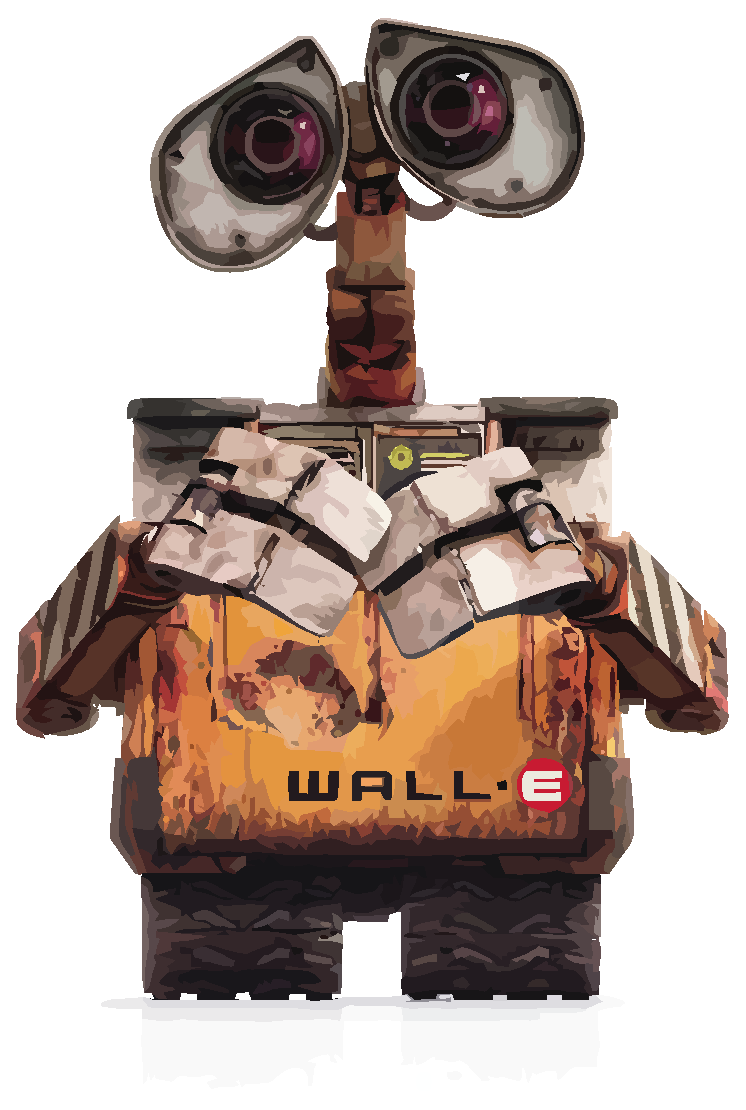
\includegraphics[width=\textwidth]{WallE}
    \caption{Wall-E}
    \label{fig:WallE}
  \end{subfigure}             
  \begin{subfigure}[b]{0.3\textwidth}
    
\includegraphics[width=\textwidth]{minion}
    \caption{Minions}
    \label{fig:Minnion}
  \end{subfigure}
  \caption{Best Animations}
  \label{fig:animations}
\end{figure}


\end{landscape}

%!TEX root = ../thesis.tex
%*******************************************************************************
%****************************** Third Chapter **********************************
%*******************************************************************************
\chapter{My third chapter}

% **************************** Define Graphics Path **************************
\ifpdf
    \graphicspath{{Chapter3/Figs/Raster/}{Chapter3/Figs/PDF/}{Chapter3/Figs/}}
\else
    \graphicspath{{Chapter3/Figs/Vector/}{Chapter3/Figs/}}
\fi

\section{First section of the third chapter}
And now I begin my third chapter here \dots

And now to cite some more people~\citet{Rea85,Ancey1996}

\subsection{First subsection in the first section}
\dots and some more 

\subsection{Second subsection in the first section}
\dots and some more \dots

\subsubsection{First subsub section in the second subsection}
\dots and some more in the first subsub section otherwise it all looks the same
doesn't it? well we can add some text to it \dots

\subsection{Third subsection in the first section}
\dots and some more \dots

\subsubsection{First subsub section in the third subsection}
\dots and some more in the first subsub section otherwise it all looks the same
doesn't it? well we can add some text to it and some more and some more and
some more and some more and some more and some more and some more \dots

\subsubsection{Second subsub section in the third subsection}
\dots and some more in the first subsub section otherwise it all looks the same
doesn't it? well we can add some text to it \dots

\section{Second section of the third chapter}
and here I write more \dots

\section{The layout of formal tables}
This section has been modified from ``Publication quality tables in \LaTeX*''
 by Simon Fear.

The layout of a table has been established over centuries of experience and 
should only be altered in extraordinary circumstances. 

When formatting a table, remember two simple guidelines at all times:

\begin{enumerate}
  \item Never, ever use vertical rules (lines).
  \item Never use double rules.
\end{enumerate}

These guidelines may seem extreme but I have
never found a good argument in favour of breaking them. For
example, if you feel that the information in the left half of
a table is so different from that on the right that it needs
to be separated by a vertical line, then you should use two
tables instead. Not everyone follows the second guideline:

There are three further guidelines worth mentioning here as they
are generally not known outside the circle of professional
typesetters and subeditors:

\begin{enumerate}\setcounter{enumi}{2}
  \item Put the units in the column heading (not in the body of
          the table).
  \item Always precede a decimal point by a digit; thus 0.1
      {\em not} just .1.
  \item Do not use `ditto' signs or any other such convention to
      repeat a previous value. In many circumstances a blank
      will serve just as well. If it won't, then repeat the value.
\end{enumerate}

A frequently seen mistake is to use `\textbackslash begin\{center\}' \dots `\textbackslash end\{center\}' inside a figure or table environment. This center environment can cause additional vertical space. If you want to avoid that just use `\textbackslash centering'


\begin{table}
\caption{A badly formatted table}
\centering
\label{table:bad_table}
\begin{tabular}{|l|c|c|c|c|}
\hline 
& \multicolumn{2}{c}{Species I} & \multicolumn{2}{c|}{Species II} \\ 
\hline
Dental measurement  & mean & SD  & mean & SD  \\ \hline 
\hline
I1MD & 6.23 & 0.91 & 5.2  & 0.7  \\
\hline 
I1LL & 7.48 & 0.56 & 8.7  & 0.71 \\
\hline 
I2MD & 3.99 & 0.63 & 4.22 & 0.54 \\
\hline 
I2LL & 6.81 & 0.02 & 6.66 & 0.01 \\
\hline 
CMD & 13.47 & 0.09 & 10.55 & 0.05 \\
\hline 
CBL & 11.88 & 0.05 & 13.11 & 0.04\\ 
\hline 
\end{tabular}
\end{table}

\begin{table}
\caption{A nice looking table}
\centering
\label{table:nice_table}
\begin{tabular}{l c c c c}
\hline 
\multirow{2}{*}{Dental measurement} & \multicolumn{2}{c}{Species I} & \multicolumn{2}{c}{Species II} \\ 
\cline{2-5}
  & mean & SD  & mean & SD  \\ 
\hline
I1MD & 6.23 & 0.91 & 5.2  & 0.7  \\

I1LL & 7.48 & 0.56 & 8.7  & 0.71 \\

I2MD & 3.99 & 0.63 & 4.22 & 0.54 \\

I2LL & 6.81 & 0.02 & 6.66 & 0.01 \\

CMD & 13.47 & 0.09 & 10.55 & 0.05 \\

CBL & 11.88 & 0.05 & 13.11 & 0.04\\ 
\hline 
\end{tabular}
\end{table}


\begin{table}
\caption{Even better looking table using booktabs}
\centering
\label{table:good_table}
\begin{tabular}{l c c c c}
\toprule
\multirow{2}{*}{Dental measurement} & \multicolumn{2}{c}{Species I} & \multicolumn{2}{c}{Species II} \\ 
\cmidrule{2-5}
  & mean & SD  & mean & SD  \\ 
\midrule
I1MD & 6.23 & 0.91 & 5.2  & 0.7  \\

I1LL & 7.48 & 0.56 & 8.7  & 0.71 \\

I2MD & 3.99 & 0.63 & 4.22 & 0.54 \\

I2LL & 6.81 & 0.02 & 6.66 & 0.01 \\

CMD & 13.47 & 0.09 & 10.55 & 0.05 \\

CBL & 11.88 & 0.05 & 13.11 & 0.04\\ 
\bottomrule
\end{tabular}
\end{table}

%\include{Chapter4/chapter4}
%\include{Chapter5/chapter5}
%\include{Chapter6/chapter6}
%\include{Chapter7/chapter7}



% ********************************** Back Matter *******************************
% Backmatter should be commented out, if you are using appendices after References
%\backmatter

% ********************************** Bibliography ******************************
\begin{spacing}{0.9}

% To use the conventional natbib style referencing
% Bibliography style previews: http://nodonn.tipido.net/bibstyle.php
% Reference styles: http://sites.stat.psu.edu/~surajit/present/bib.htm

\bibliographystyle{apalike}
%\bibliographystyle{unsrt} % Use for unsorted references  
%\bibliographystyle{plainnat} % use this to have URLs listed in References
\cleardoublepage
\bibliography{References/references} % Path to your References.bib file


% If you would like to use BibLaTeX for your references, pass `custombib' as
% an option in the document class. The location of 'reference.bib' should be
% specified in the preamble.tex file in the custombib section.
% Comment out the lines related to natbib above and uncomment the following line.

%\printbibliography[heading=bibintoc, title={References}]


\end{spacing}

% ********************************** Appendices ********************************

\begin{appendices} % Using appendices environment for more functunality

%!TEX root = ../thesis.tex
% ******************************* Thesis Appendix A ****************************
\chapter{Detailed breakdown of systematic uncertainties} 
\label{app:uncert}

\begin{longtable}{ l | c | c | c }%[htbp!]
%\center
\caption{Extracted cross sections with detailed
  list of uncertainties. Besides the contribution to the total
  uncertainty in \%, the fitted value of the nuisance parameter (pull), as well as the ratio of the estimated
  uncertainty over the uncertainty from a 1 $\sigma$ variation, called
  constr/$\sigma$, are shown. 
  \label{tab:lh_res_eightfull}}\\
\hline
Name & Pull & Constr / $\sigma$ & Contribution [\%] \\ 
\hline
\endfirsthead
\hline
Name & Pull & Constr / $\sigma$ & Contribution [\%] \\ 
\hline
\endhead
B-tag & 0.617 & 0.49 & ${0.456}$ \\
Mistag & 0.413 & 0.96 & ${0.129}$ \\
DY ME scale & -0.583 & 0.44 & ${0.118}$ \\
Electron energy resolution & -0.076 & 0.91 & ${-0.007}$ \\
Electron energy scale & -1.271 & 0.63 & ${-0.015}$ \\
Electron ID & 0.291 & 0.6 & ${-1.907}$ \\
Jet energy resolution & 1.096 & 0.81 & ${-0.008}$ \\
JES: MPF & 0.101 & 0.66 & ${0.002}$ \\
JES: Absolute Scale & -0.053 & 0.77 & ${0.019}$ \\
JES: Absolute Stat & 0.266 & 0.83 & ${-0.039}$ \\
JES\_Fragmentation & 0.203 & 0.63 & ${-0.038}$ \\
JES: Pileup Data/MC & -0.265 & 0.89 & ${-0.063}$ \\
JES: Pileup $p_T$ BB & 0.166 & 0.75 & ${-0.093}$ \\
JES\_PileUpPtEC1 & -0.12 & 0.65 & ${-0.046}$ \\
JES\_PileUpPtRef & 0.28 & 0.56 & ${-0.084}$ \\
JES\_RelativeBal & -0.709 & 0.52 & ${0.143}$ \\
JES: Intercalibration & 0.068 & 0.66 & ${-0.001}$ \\
JES: Relative JER EC1 & -0.074 & 1.03 & ${0.008}$ \\
JES: Relative $p_T$ BB & -0.025 & 0.87 & ${0.019}$ \\
JES: Relative $p_T$ EC1 & -0.012 & 0.91 & ${-0.049}$ \\
JES\_RelativeStatEC & 0.296 & 0.73 & ${-0.026}$ \\
JES\_RelativeStatFSR & -0.085 & 1.07 & ${0.033}$ \\
JES: Single pion ECAL & 0.264 & 0.6 & ${-0.060}$ \\
JES: Single pion HCAL & 0.171 & 0.63 & ${-0.026}$ \\
JES\_TimePtEta & 0.255 & 0.68 & ${-0.019}$ \\
Muon energy scale & 0.114 & 0.99 & ${0.043}$ \\
Muon ID & -0.343 & 0.84 & ${-2.021}$ \\
Pile-up & 0.511 & 0.82 & ${0.312}$ \\
top mass & 0 & 0 & ${0.000}$ \\
Top $p_{T}$ & 1 & 0.74 & ${-0.001}$ \\
Trigger & -0.022 & 0.99 & ${-0.645}$ \\
B-hadron BR & 0.093 & 0.72 & ${0.075}$ \\
TT\_CRERD & 0 & 0.69 & ${0.000}$ \\
TT\_CRGLUON & 0.184 & 0.17 & ${0.006}$ \\
TT\_CRQCD & 0.105 & 0.12 & ${0.139}$ \\
fragm. Peterson & 0.521 & 0.41 & ${0.302}$ \\
fragmentation & -0.768 & 0.58 & ${-0.694}$ \\
$t\bar{t}$/tW FSR scale & -0.201 & 0.17 & ${0.560}$ \\
NLO generator & 0 & 0 & ${0.000}$ \\
$t\bar{t}$/tW ISR scale & 0.111 & 0.18 & ${-0.305}$ \\
ME/PS matching & -0.138 & 0.2 & ${0.148}$ \\
$t\bar{t}$ ME scale & 1 & 0.32 & ${0.000}$ \\
UE tune & 0.163 & 0.26 & ${0.180}$ \\
PDF10 & -0.065 & 0.84 & ${0.367}$ \\
PDF11 & -0.003 & 0.86 & ${0.139}$ \\
PDF12 & 0.022 & 0.86 & ${-0.209}$ \\
PDF13 & 0.21 & 0.85 & ${0.155}$ \\
PDF14 & 0.06 & 0.87 & ${-0.082}$ \\
PDF15 & 0.061 & 0.83 & ${-0.051}$ \\
PDF16 & 0.004 & 0.86 & ${0.061}$ \\
PDF17 & -0.043 & 0.85 & ${-0.150}$ \\
PDF18 & -0.228 & 0.85 & ${0.021}$ \\
PDF19 & -0.106 & 0.82 & ${0.257}$ \\
PDF1 & -0.018 & 0.88 & ${-0.037}$ \\
PDF20 & 0.002 & 0.83 & ${0.098}$ \\
PDF21 & -0.115 & 0.86 & ${-0.173}$ \\
PDF22 & -0.239 & 0.85 & ${-0.223}$ \\
PDF23 & 0.096 & 0.76 & ${-0.008}$ \\
PDF24 & 0.104 & 0.87 & ${0.137}$ \\
PDF25 & -0.083 & 0.83 & ${-0.020}$ \\
PDF26 & 0.013 & 0.83 & ${0.021}$ \\
PDF27 & -0.045 & 0.88 & ${0.092}$ \\
PDF28 & 0.035 & 0.85 & ${-0.011}$ \\
PDF2 & -0.241 & 0.97 & ${-0.047}$ \\
PDF3 & -0.005 & 0.86 & ${0.147}$ \\
PDF4 & -0.092 & 0.92 & ${0.071}$ \\
PDF5 & 0.085 & 0.8 & ${-0.329}$ \\
PDF6 & -0.006 & 0.87 & ${0.109}$ \\
PDF7 & 0.16 & 0.78 & ${-0.385}$ \\
PDF8 & 0.046 & 0.85 & ${-0.026}$ \\
PDF9 & -0.084 & 0.85 & ${-0.014}$ \\
JES: Flavor response & -0.335 & 0.63 & ${-0.076}$ \\
tW background & -0.422 & 0.46 & ${-0.815}$ \\
Diboson background & 0.849 & 0.78 & ${0.206}$ \\
W+jets background & -0.905 & 0.83 & ${0.036}$ \\
$t\bar{t}$ background & 0.102 & 0.98 & ${-0.084}$ \\
DY background (0 b-jets) & -0.045 & 0.36 & ${0.430}$ \\
DY background (1 b-jets) & -0.429 & 0.22 & ${0.172}$ \\
DY background (2 b-jets) & -0.643 & 0.78 & ${-0.014}$ \\
Stat &  &  & ${0.252}$ \\
Total vis &  &  & $\pm^{2.648}_{2.549}$ \\ \hline
$\sigma_{t\bar{t}}$(13 TeV) vis &   &   & 28.1033 pb \\ \hline
$t\bar{t}$/tW ISR scale (extr) &  &  & $\mp^{0.146}_{0.105}$ \\
$t\bar{t}$/tW FSR scale (extr) &  &  & $\pm^{0.084}_{0.065}$ \\
$t\bar{t}$ ME scale (extr) &  &  & $\mp^{0.392}_{0.000}$ \\
UE tune (extr) &  &  & $\mp^{0.188}_{0.053}$ \\
PDF (extr) &  &  & $\pm^{0.818}_{0.588}$ \\
Top $p_{T}$ (extr) &  &  & $\pm^{0.000}_{0.446}$ \\ \hline
Total &  &  & $\pm^{2.810}_{2.654}$ \\ \hline
$\sigma_{t\bar{t}}$(13 TeV) &   &   & 819.95 pb \\ \\ \hline \hline

\end{longtable}
%!TEX root = ../thesis.tex
% ******************************* Thesis Appendix B ********************************

\chapter{List of publications}

\begin{itemize}

\item Measurement of the top quark pair production cross section at 13 TeV with the CMS detector, \\
T. Arndt, PoS TOP2015 (2016) 026

\item Measurement of the top quark pair production cross section using e$\mu$ events in proton-proton
collisions at $\sqrt{s}= 13 \TeV$ with the CMS detector, \\
CMS Collaboration, Eur.Phys.J. C77 (2017) 172, DOI: 10.1140/epjc/s10052-017-4718-8

\item Measurement of the top quark pair production cross section in proton-proton collisions at $\sqrt{s}= 13 \TeV$ with the CMS detector, \\
CMS Collaboration, Phys. Rev. Lett. 116 (2016) 052002, DOI: 10.1103/PhysRevLett.116.052002

\item Measurement of normalized differential tt cross sections in the dilepton channel from pp
collisions at $\sqrt{s}= 13 \TeV$, \\
CMS Collaboration, JHEP 1704 (2017) 060, DOI: 10.1007/JHEP04(2018)060

\item Search for $\ttbar\mathrm{H}$ production in the $\mathrm{H}\rightarrow\mathrm{b}\bar{\mathrm{b}}$ decay channel with leptonic \ttbar decays in proton-proton
collisions at $\sqrt{s}= 13 \TeV$, \\
CMS Collaboration, Preliminary publication, April 2018, CMS-PAS-HIG-17-026

\item Search for $\ttbar\mathrm{H}$ production in the $\mathrm{H}\rightarrow\mathrm{b}\bar{\mathrm{b}}$ decay channel with $\sqrt{s}= 13 \TeV$ pp collisions at the CMS
experiment,\\
CMS Collaboration, Preliminary publication, March 2016, CMS-PAS-HIG-16-004

\item First measurement of the differential cross section for \ttbar production in the dilepton final
state at $\sqrt{s}= 13 \TeV$, \\
CMS Collaboration, Preliminary publication, August 2015, CMS-PAS-TOP-15-010

\end{itemize}




\end{appendices}

% *************************************** Index ********************************
\printthesisindex % If index is present

\end{document}
